\chapter{Математическая постановка задачи}
\label{ch:math}

\todo{Не уверен насчет названия главы}

\section{Теория типов}
\label{sec:type_theory}

В разделе представлена информация о специальном разделе математики - теории типов~\cite{TypeTheoryBook}.
Освещены важные понятия - \textit{терм}, \textit{тип}, \textit{суждение} и \textit{система типов}.

Теория типов является альтернативой для теории множеств и теории категорий.
В отличие от остальных, она позволяет исследовать свойства объекта, учитывая его структуру, а не множество, которому он принадлежит.
Поэтому теория типов нашла свое применение в программировании, в частности, в компиляторах в фазе статического анализа программы, как для вывода, так и для проверки соответствия типов.
Более того, согласно изоморфизму Карри-Ховарда~\cite{TypeTheoryArticle} (таблица \ref{tab:curry-hovard-iso}), программы могут быть использованы для доказательства логических высказываний.
Такие доказательства называют автоматическими, и они широко применяется среди таких языков, как Agda, Coq, Idris.

Терм $x$ - чаще всего элемент языка программирования, будь то переменная, константа, вызов функции и др.
Термы могут включать в себя другие термы.
Например, термом является конструкция $(x + 1) * (x + 1)$, построенная из других термов: $x$, $1$, $+$ и $*$.

Типом $A$ обозначается метка, например объекты на натюрмортах принадлежат к типу (классу) <<фрукты>>.
Обычно каждому терму соответствует определенный тип - $x: A$.
Типы позволяют строго говорить о возможных действиях над объектом, а также формализовать взаимоотношения между ними.

Система типов определяет правила взаимодействия между типами и термами.
В программировании это понятие равноценно понятию типизация.

Кроме того, также используются такие термины, как \textit{суждения} и \textit{предположения}.
С помощью суждений (англ. judgments) можно создавать логические конструкции: выражение $\vdash x: T$ говорит, что терм $x$ имеет тип $T$.
Слева от знака $\vdash$ записывается контекст: $x: integer \vdash (x + 1): integer$ - если терм $x$ имеет тип числа, то $x + 1$ тоже имеет тип числа.
Таким образом, суждение обозначается так:

\begin{equation}
    \Gamma \vdash P,
    \label{eq:judgment}
\end{equation}
где $\Gamma$ - контекст,\\$P$ - предположение.

Всего существует 6 видов суждений:

\begin{table}[h]
    \centering
    \label{tab:types_of_judgments}
    \begin{tabular}{l r}
        $\Gamma \vdash$                  & $\Gamma$ - верный контекст,                  \\
        $\Gamma \vdash \tau$             & $\tau$ - тип в контексте,                    \\
        $\Gamma \vdash x: \tau$          & терм $x$ имеет тип $\tau$ в контексте,       \\
        $\vdash \Gamma = \Delta$         & контексты $\Gamma$ и $\Delta$ равны,         \\
        $\Gamma \vdash \tau_1 = \tau_2$  & типы $\tau_1$ и $\tau_2$ в контексте равны,  \\
        $\Gamma \vdash x_1 = x_2 : \tau$ & терм $x_1$ равен терму $x_2$ с типом $\tau$.
    \end{tabular}
\end{table}

\begin{table}[h]
    \centering
    \caption{Изоморфизм Карри-Ховарда}
    \label{tab:curry-hovard-iso}
    \begin{tabular}{|c|c|}
        \hline
        \textbf{Логическое высказывание} & \textbf{Язык программирования} \\\hline
        Высказывание, $F$, $Q$           & Тип, $A$, $B$                  \\\hline
        Доказательство высказывания $F$  & $x: A$                         \\\hline
        Высказывание доказуемо           & Тип $A$ обитаем                \\\hline
        $F \implies Q$                   & Функция, $A \to B$             \\\hline
        $F \wedge Q$                     & Тип-произведение, $A \times B$ \\\hline
        $F \vee Q$                       & Тип-сумма, $A + B$             \\\hline
        Истина                           & Единичный тип, $\top$          \\\hline
        Ложь                             & Пустой тип, $\bot$             \\\hline
        $\neg F$                         & $A \to \bot$                   \\\hline
    \end{tabular}
\end{table}

Тип $T$ обитаем (англ. inhabitat), если выполняется следующее: $\exists t: \Gamma \vdash t: T$ - найдется терм $t$, такой, что в контексте $\Gamma$ он будет иметь тип $T$.

Из одних суждений можно получить другие суждения по определенным правилам.
Такие правила называются \textit{правилами вывода} и выглядят следующим образом: $\displaystyle \frac{J_1}{J_2}$, что означает если верно суждение $J_1$, то и верно суждение $J_2$.
Таким образом из правил вывода получаются деревья вывода, где каждое входное суждение $J_1$ заменяется правилом вывода.
Например, следующее правило определяет тип применения функции $f$ к аргументу $x$:

\begin{equation}
    \label{eq:judgement_substitution}
    \frac{\Gamma \vdash x: T_1, f: T_1 \to T_2}{\Gamma \vdash f(x): T_2}
\end{equation}

Выражение~\ref{eq:judgement_substitution} можно трактовать следующим образом: если в контексте $\Gamma$ терм $x$ имеет тип $T_1$, а терм $f$ - $T_1 \to T_2$ (функциональный тип), то можно судить, что терм $f(x)$ (применение функции) имеет тип $T_2$.

%----------------------------------------------------------

\section{Классификация систем типов}
\label{sec:classification}
%----------------------------------------------------------

Известно, что системы типов можно разделить на \textit{динамические} и \textit{статические}~\cite{Typing}.
Это влияет на то, в какой момент в программе происходит проверка соответствия типов.
В динамических системах - во время исполнения программы, а в статических - соответственно во время компиляции.
Кроме того, существуют особые языки программирования, где все данные имеют один тип.
К таким относятся многие низкоуровневые языки, например ассемблер.
Все данные в нем (адреса в памяти, числа, указатели на функции) являются всего лишь последовательностью байт.

Ниже приведены основные критерии, по которым можно классифицировать систему типов в языках программирования:

\begin{enumerate}[1)]
    \item по времени проверки соответствия типам: статическая и динамическая,
    \item по поддержке неявных конверсий: сильная (англ. strong) и слабая,
    \item по необходимости вручную типизировать выражение: явная и неявная.
\end{enumerate}

Например, типизация в язык python является динамической, сильной и неявной с точки зрения этой классификации~\cite{PythonWiki}.
Интерпретатор знает тип переменной только во время выполнения и не может неявно изменить его.

Статические системы типов обладают несомненным преимуществом, по сравнению с динамическими - компилятор может использовать накопленную во время семантического анализа информацию для оптимизации кода.
Но необходимо учитывать, что такая типизация вносит некоторые неудобства: программисту постоянно приходится прилагать усилия по устранению ошибок, связанных с типами.
Это делает языки со статической типизацией, хоть и более сложными в использовании, но более быстрыми, а динамически типизированным языкам приходится использовать различные специфические оптимизации вроде \textit{JIT-компиляции}, чтобы добиться сопоставимой производительности.

JIT-компиляцией (just-in-time компиляцией) называется прием оптимизации при выполнении программы, когда компиляция происходит во время работы программы.
Она была создана, чтобы решить проблемы с производительностью при интерпретации кода.

Проанализируем системы типов, используемые в некоторых современных языках программирования с целью выявить их сильные и слабые стороны.
\todo{дополнить?}

\subsection{Система типов C}
\label{subsec:c_type_system}

C - язык программирования со статической, слабой, явной типизацией, разработанный в 1970-х годах.

Типом в языке C является интерпретация набора байт, составляющих объект~\cite{CSpec}.
Все типы бывают двух видов: базовые и производные (рис. \ref{fig:c_types}).
Также их можно разделить на две группы: скалярные и агрегатные.

В группу скалярных типов относят примитивные (базовые) типы и указатели.
Базовые типы в свою очередь делятся на целые и вещественные числа.
Указатели - тоже скалярная величина, их размер зависит от архитектуры системы.

В группу агрегатных относятся структуры и массивы.
Они позволяют определить тип, который включает в себя несколько других.

Кроме того, существуют <<специальные>> типы - объединения и указатели на функции.
С помощью объединений можно задать варианты представления данных (листинг~\ref{lst:union}).

\begin{figure}[H]
    \centering
    \import{figures/.generated/}{c_types.pdf_tex}
    \caption{Схематичное изображение типов в C}
    \label{fig:c_types}
\end{figure}

\begin{lstlisting}[label={lst:union},language=C,caption={Объявление безымянного объединения в языке C. В одной переменной твкого типа может содержаться либо целое число, либо вещественное.}]
union {
    int first_variant;
    float second_variant;
};
\end{lstlisting}

Достоинства:
\begin{itemize}
    \item C прост для понимания, он содержит только основные типы данных,
    \item язык позволяет эффективно работать с данными в том виде, как они реализованы в ЭВМ.
\end{itemize}

Недостатки:
\begin{itemize}
    \item недостаточная выразительность по сравнению с другими языками программирования,
    \item мало гарантий и проверок, осуществляемых компилятором (\ref{lst:weak_c}).
\end{itemize}

Здесь под выразительностью стоит понимать то, насколько много идей можно реализовать и насколько лаконично они при этом будут выглядеть.
Например, хоть в C и можно выразить идею объекто-ориентированного программирования, но это будет выглядеть гораздо более громоздко, чем в C++~\cite{OOP_in_C}.

\begin{lstlisting}[label={lst:weak_c},language=C,caption={Неправильное использование \lstinline{void*} не может быть отслежено компилятором}]
// компилятор не знает исходный тип аргумента
long* foo(void* arg) { return (long*) arg; }

int main() {
    void *value = &foo;
    long result = (*foo(value)) + 1; // неопределенное поведениe
}
\end{lstlisting}

\subsection{Система типов Java}
\label{subsec:java_type_system}

Язык Java разработан компанией Sun Microsystems в 1995 году.
Благодаря использованию дополнительной абстракции в виде виртуальной машины, может выполняться на большом количестве архитектур ЭВМ.
Популярен среди разработчиков самых разных областей: от банковского сектора до приложений под ОС Android.

Систему типов, применяемую в этом языке можно охарактеризовать как статическую, сильную и явную с возможностью введения неявно типизированных выражений~\cite{JavaTypeSystem}.
Java создавалась под сильным влиянием идей объектно-ориентированного программирования, поэтому она включает классы, интерфейсы, обобщения и прочее.
Язык эволюционировал, но пытался сохранить обратную совместимость с прошлыми версиями, поэтому имеются и недостатки - вся информация об обобщенной переменной стирается во время исполнения программы.
Это иногда приводит к ошибкам при работе с коллекциями.

Все типы делятся на примитивные и объектные (пользовательские).
Их различает значение по-умолчанию: в случае пользовательских - \lstinline{null}, примитивных - в зависимости от типа.
К примитивным типам относятся различные виды представления чисел, символы и логический тип.
Для использования примитивных типов в коллекциях, используется упаковка (англ. boxing).
Суть её заключается в том, что значение такого типа <<упаковывается>> в соответствующий объектный тип, который представляет собой указатель на значение вместе с метаданными.

Достоинства:
\begin{itemize}
    \item наличие в системе типов обобщений позволяет уменьшить количество повторяемого кода,
    \item поддержка некоторых особенностей динамической типизации, при преобладании статической.
\end{itemize}

Недостатки:
\begin{itemize}
    \item из-за специфики работы обобщенных типов в виртуальной машине Java, могут возникать ошибки с приведением типов,
    \item из-за разделения на примитивные и объектные типы, а также дополнительных затрат на упаковку, ухудшается производительность,
    \item избыточность определений типов в очевидных местах; хоть это и было исправлено в последующих версиях языка с помощью локального вывода типов, синтаксис языка все ещё перегружен.
\end{itemize}

\subsection{Система типов ML-подобных языков}
\label{subsec:ml_type_system}

\todo{пояснить, почему именно эту юзаем}

К семейству ML-подобных языков относят функциональные языки с развитой системой типов.
В основе неё лежит типизированное лямбда-исчисление.
Это формализованная система для описания программ, предложенная Алонзо Чёрчем в 1930 году и в отличие от обычного лямбда-исчисления, здесь каждому терму сопоставлен тип.

Кроме проверки типов, над такими системами можно удобно проводить \textit{вывод типов}.
Это позволяет пользователю составлять программы почти не используя аннотации типов.

Алгоритмы вывода типов позволяют компилятору узнать тип терма из контекста.

\todo{переписать более понятным языком}

Лямбда-куб позволяет наглядно увидеть разницу и взаимоотношение между различными видами тизипированными лямбда-исчислениями (рис. \ref{fig:lambda_cube}).

\todo{terrible picture}
\begin{figure}[H]
    \centering
    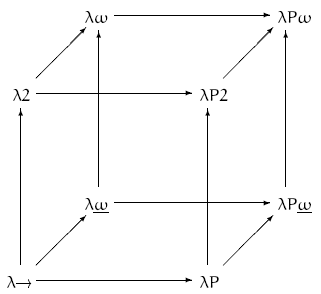
\includegraphics{figures/Lambda_cube}
    \caption{Графическое изображение лямбда-куба}
    \label{fig:lambda_cube}
\end{figure}

Простейшим вариантом является \textit{просто типизированное лямбда-исчисление} ($\lambda \to$).
В нем доступна абстракция только с помощью функции:

\begin{equation}
    \label{eq:STLC}
    \frac{\Gamma \cup x: T \vdash y: U}{\Gamma \vdash \lambda x.y: T \to U}
\end{equation}

Следующим этапом является \textit{полиморфное лямбда-исчисление} ($\lambda 2$).
В нём термы могут зависеть от типов (обобщенные функции):

\begin{equation}
    \label{eq:2TLC}
    \frac{\Gamma \vdash y: U}{\Gamma \vdash \forall T: \lambda (x: T).y: T \to U}
\end{equation}

Еще одним расширением будет \textit{лямбда-исчисление с операторами над типами} ($\lambda \underline{w}$).
С точки зрения обычных языков программирования такое исчисление формирует функции над типами:
В частности, функция, формирующая тип списка, выглядела бы так:

\begin{equation}
    \label{eq:WTLC}
    \lambda \alpha: *. \alpha \to List ~\alpha,
\end{equation}
где $*$ - любой другой тип

Последней простой точкой куба является \textit{лямбда-исчисление с зависимыми типами} ($\lambda P$).
Оно примечательно тем, что типы могут зависеть от термов.
Наиболее простым примером послужит функция деления, где входной аргумент обязан быть отличным от $0$.

Остальные вершины являются комбинацией описанных систем.

Подведем итог.

Достоинства:
\begin{itemize}
    \item выразительность системы типов легко показать том же самом лямбда-кубе,
    \item имеет строгое математическое обоснование и хорошо изучено,
    \item компилятор имеет возможность выявить больше ошибок в программе.
\end{itemize}

Недостатки:
\begin{itemize}
    \item достаточно сложна для понимания как с точки зрения пользователя, так и разработчика компилятора
    \item может значительно увеличить время компиляции из-за обилия сложных алгоритмов
\end{itemize}

%----------------------------------------------------------

\section{Система типов Хиндли-Милнера}
\label{sec:hindley-milner}

\todo{может по-другому назвать секцию, я юзаю kinda свою систему типов}

Для начала определим термы:

\begin{equation}
    \label{eq:terms}
    \begin{aligned}
        e_1, e_2, e_3 \coloneqq ~ &x \\
        &| ~ e_1(e_2) \\
        &| ~ \lambda x : \tau. e_1 \\
        &| ~ \text{let } x: \tau = e_2 \text{ in } e_2 \\
        &| ~ \text{:num:} \\
        &| ~ (e_1, e_2) \\
        &| ~ \text{if } e_1 \text{ then } e_2 \text{ otherwise } e_3,
    \end{aligned}
\end{equation}
где $e_1, e_2, e_3$ - термы,\\
$x$ - имя переменной (англ. binding), :num: - числовой литерал,\\
$\tau$ - тип.

Поясним значение каждого варианта терма подробнее.

\begin{enumerate}
    \item Переменная позволяет сослаться на другое имя, определенное выше по тексту программы, например на функцию или другую переменную.
    \item Запись $e_1(e_2)$ обозначает применение функции ($e_1$) к ее аргументу ($e_2$).
    Проще говоря - вызов функции.
    \item $\lambda x: \tau. e_1$ означает создание безымянной, лямбда, функции.
    \item Объявление новых переменных происходит с помощью конструкции $\text{let } \ldots \text{ in } \ldots$.
    \item Последняя конструкция необходима для создания пар из двух других термов.
\end{enumerate}

В некоторых элементах к переменной $x$ приписывается ограничение на тип $\tau$.
Это необходимо для того, чтобы явно указать необходимый тип, как это делается в других языках программирования (листинг~\ref{lst:type_bound}).

\begin{lstlisting}[label={lst:type_bound},language=C,caption={Явное указание типа аргумента в языке C.}]
    void foo(int a) { }
\end{lstlisting}

Теперь можно ввести определение типа $\tau$.

\begin{equation}
    \label{eq:types}
    \begin{aligned}
        \tau_1, \tau_2 \coloneqq ~ &\text{Integer} ~|~ \text{Real} ~|~ \text{Boolean} \\
        &| ~ \alpha \\
        &| ~ \tau_1 \to \tau_2 \\
        &| ~ (\tau_1, \tau_2, \ldots, \tau_n) \\
        &| ~ C,
    \end{aligned}
\end{equation}
где $C$ - имя типа (константа), определенное пользователем,\\
$\alpha$ - переменная типа,\\
Integer, Real, Boolean - примитивные типы для целых, вещественных и логических данных соответственно.

Переменная типа необходима для тех же целей, что и обычная переменная: она может ссылаться на другой тип или быть любым типом.
Под записью $(\tau_1, \tau_2, \ldots, \tau_n)$ стоит понимать тип-кортеж, образованный несколькими другими типами.

Также к обычным типам необходимо добавить так называемые \textit{полиморфные} типы~\eqref{eq:poly_types}.
Они необходимы для введения квантора всеобщности по отношению к переменным типа.
С точки зрения обычных языков программирования, такие полиморфные типы можно оценивать как обобщенные типы (листинг~\ref{lst:generics}).

\begin{equation}
    \label{eq:poly_types}
    \sigma \coloneqq \tau ~|~ \forall A. \sigma,
\end{equation}
где $A = \left\{ \alpha \right\}$ - неупорядоченное множество переменных типа.

\begin{lstlisting}[language=C++,label=lst:generics,caption={Определение обобщенной функции в C++}]
    template<typename T>
    void foo(T value) {}
\end{lstlisting}

Далее введем следующие понятия:
\textit{контекст} $\Gamma$~\eqref{eq:context},
множество \textit{свободных типов} (англ. free types)~\eqref{eq:free_types},
\textit{обобщение} (англ. generalize)~\eqref{eq:generalize},
\textit{подстановка} (англ. substitutions)~\eqref{eq:subst} и
\textit{конкретизация} (англ. instantiate)~\eqref{eq:instantiate}.
В скобках указан номер выражения, содержащего необходимое определение.

\begin{equation}
    \label{eq:context}
    \Gamma = \left\{ x: \sigma ~|~ x \in X, \sigma \in \Sigma \right\},
\end{equation}
где $X$ - множество термов,\\
$\Sigma$ - множество полиморфных типов.

\begin{equation}
    \label{eq:free_types}
    \begin{aligned}
        ft(\sigma) &= ft(\tau) \backslash A, \\
        ft(\tau)   &= \left\{ \alpha ~|~ \alpha \in \tau \right\}, \\
        ft(\Gamma) &= \bigcup_{x: \sigma \in \Gamma} ft(\sigma)
    \end{aligned}
\end{equation}
где $\alpha \in \tau$ - переменная типа, использованная в типе $\tau$,\\
$X \backslash Y$ - множество $X$, исключая элементы множества $Y$.

\begin{equation}
    \label{eq:generalize}
    gn(\Gamma, \tau) = \forall A. \tau,
\end{equation}
где $A = ft(\tau) \backslash ft(\Gamma)$.

\begin{equation}
    \label{eq:subst}
    \mathcal{S} = \left[ \alpha_1 \coloneqq \tau_1, \alpha_2 \coloneqq \tau_2, \ldots \alpha_n \coloneqq \tau_n \right],
\end{equation}
где ни одна пара $\alpha_i \coloneqq \tau_i$ не должна быть вида $\alpha_i \coloneqq \alpha_i$, иначе будет получена подстановка для бесконечно рекурсивного типа.

Композиция подстановок:

\begin{equation}
    \label{eq:subst_comp}
    \mathcal{S}_1 \circ \mathcal{S}_2 = \mathcal{S}_1 \cup \left[ \alpha_i \coloneqq \mathcal{S}_1 \tau_i \right]
\end{equation}

Применение подстановки $\mathcal{S} \tau$ - операция замены всех вхождений очередной $\alpha_i$ из подстановки $\mathcal{S}$ на $\tau_i$ в типе $\tau$.

Будем называть $\beta$ - уникальную переменную типа.

\begin{equation}
    \label{eq:instantiate}
    it(\sigma) = \mathcal{S}_{\sigma} \tau,
\end{equation}
где $\mathcal{S}_\sigma = \left[ \alpha \coloneqq \beta ~|~ \alpha \in A, \beta \ne \alpha \right]$.

Правила вывода, разработанные Милнером~\cite{UrbanN2009}, позволяют получить доказательство, что любой терм, заданный выражением~\eqref{eq:terms} можно типизировать определенным типом.
Алгоритм, построенный с такими правилами, называется алгоритмом $\mathcal{W}$.
Одним из его недостатков является неточное определение места ошибки при типизации выражения.
Вместо него предлагается использовать модификацию этого алгоритма с использованием ограничений (англ. constraints) и отложенной унификацией.

Унификацией называется процесс поиска такой подстановки $\mathcal{S}$ для двух типов $\tau_1$ и $\tau_2$, что $\mathcal{S} \tau_1 = \mathcal{S} \tau_2$.
Для решения этой задачи существует алгоритм $\mathcal{U}$:

\begin{equation}
    \label{eq:algo_u}
    \begin{aligned}
        \mathcal{U}(\tau_1, \tau_1) &= \left[  \right], \\
        \mathcal{U}(\alpha_1, \tau_2) &= \left[ \alpha_1 \coloneqq \tau_2 \right] \text{ если } \alpha_1 \notin \tau_2, \\
        \mathcal{U}(\tau_1, \alpha_2) &= \left[ \alpha_2 \coloneqq \tau_1 \right] \text{ если } \alpha_2 \notin \tau_1, \\
        \mathcal{U}(\tau^{in}_1 \to \tau^{out}_1, \tau^{in}_2 \to \tau^{out}_2) &= \mathcal{U}(\tau^{in}_1, \tau^{in}_2) \cup \mathcal{U}(\tau^{out}_1, \tau^{out}_2), \\
        \mathcal{U}((\tau_1^A, \ldots, \tau_n^A), (\tau_1^B, \ldots, \tau_n^B)) &= \bigcup_{i = 1}^{n} \mathcal{U}(\tau_i^A, \tau_i^B)
    \end{aligned}
\end{equation}

\section{Использование ограничений при выводе типов}
\label{sec:constratints_usage}

Алгоритм вывода типов, использующий ограничения - алгоритм $\mathcal{W}_c$ - имеет, по сравнению с алгоритмом $\mathcal{W}$, два основных преимущества:
\begin{itemize}
    \item он использует отложенную унификацию и вместо нее работает с ограничениями, а не с подстановками, что позволяет выводить тип для более узких случаев,
    \item ему не нужен глобальный контекст при выводе типа - всю требуемую информацию он сохраняет в ограничениях и \textit{множестве предположений}.
\end{itemize}

Под ограничением $c$ будем понимать следующее определение:

\begin{equation}
    \label{eq:cst}
    \begin{aligned}
        c \coloneqq ~ &\tau_1 \equiv \tau_2, \\
        &| ~ \tau_1 \leq_{\mathcal{M}} \tau_2, \\
        &| ~ \tau \preceq \sigma
    \end{aligned}
\end{equation}

\begin{itemize}
    \item Ограничение эквивалентности ($\tau_1 \equiv \tau_2$) говорит, что типы $\tau_1$ и $\tau_2$ должны быть унифицированы.
    \item Явное ограничение на экземпляр ($\tau \preceq \sigma$) указывает, что тип $\tau$ должен быть каким-то конкретным экземпляром полиморфного типа $\sigma$.
    \item Неявное ограничение на экземпляр ($\tau_1 \leq_{\mathcal{M}} \tau_2$) показывает, что тип $\tau$ должен быть конкретным экземпляром типа, полученного после обобщения типа $\tau_2$ в контексте $\mathcal{M}$.
\end{itemize}

Последние два ограничения возникают из-за полиморфных свойств объявления переменной.
А именно - тип переменной $x$ в выражении $\text{let } x = e_1 \text{ in } e_2$ должен быть конкретным экземпляром полиморфного типа для каждого места использования.
Явное ограничение на экземпляр не подходит, так как на момент обработки выражения тип $e_1$ не может быть полиморфным.
Поэтому необходимо использовать неявное ограничение, контекст $\mathcal{M}$ которого пополняется по ходу выполнения алгоритма.

Правила вывода, используемые в алгоритме $\mathcal{W}_c$, состоят из суждений вида $\mathcal{A}, \mathcal{C} \vdash e: \tau$, где $\mathcal{A}$ - множество предположений, $\mathcal{C}$ - ограничения, $e$ - терм, $\tau$ - тип.
Сами правила представлены в подразделе~\ref{subsec:inference_rules}
В отличие от контекста $\Gamma$, используемом в алгоритме $\mathcal{W}$, в множество предположений для каждой переменной сохраняется набор её возможных типов~\eqref{eq:assumption_set}.
Кроме того, при рекурсивном применении правил, множества предположений просто соединяются между собой.

\begin{equation}
    \label{eq:assumption_set}
    \mathcal{A} = \left\{ x: T ~|~ x \in X \right\},
\end{equation}
где $X$ - множество переменных,\\
$T = \left\{ \tau_1, \tau_2, \ldots, \tau_n \right\}$ - множество возможных типов.

Неявное ограничение на экземпляр использует контекст $\mathcal{M}$.
Он может быть получен для каждого терма $e$ следующим образом:

\begin{equation}
    \label{eq:monomorphic_set}
    \begin{aligned}
        \mathcal{M}(x) &= \emptyset, \\
        \mathcal{M}(e_1(e_2)) &= \mathcal{M}(e_1) \cup \mathcal{M}(e_2), \\
        \mathcal{M}(\lambda x: \tau. e_1) &= \left\{ \beta \right\} \cup \mathcal{M}(e_1), \\
        \mathcal{M}(\text{let } x: \tau = e_1 \text{ in } e_2) &= \mathcal{M}(e_1) \cup \mathcal{M}(e_2), \\
        \mathcal{M}(\text{:num:}) &= \emptyset, \\
        \mathcal{M}((e_1, e_2)) &= \mathcal{M}(e_1) \cup \mathcal{M}(e_2), \\
        \mathcal{M}(\text{if } e_1 \text{ then } e_2 \text{ otherwise } e_3) &= \mathcal{M}(e_1) \cup \mathcal{M}(e_2) \cup \mathcal{M}(e_3), \\
    \end{aligned}
\end{equation}

\subsection{Правила вывода}
\label{subsec:inference_rules}

Каждое правило записано одним выражением в том виде, который определен в разделе~\ref{sec:type_theory}.
Для каждого варианта терма определено собственное правило.
Таким образом любой терм может быть типизирован.

Правило для варианта терма $e = x$:

\begin{equation}
    \label{eq:var_infer}
    \frac{}{\left\{ x: \left\{ \beta \right\} \right\}, \emptyset \vdash e: \beta}
\end{equation}

Правило для варианта терма $e = e_1(e_2)$:

\begin{equation}
    \label{eq:app_infer}
    \frac{
        \mathcal{A}_1, \mathcal{C}_1 \vdash e_1: \tau_1 ~~ \mathcal{A}_2, \mathcal{C}_2 \vdash e_2: \tau_2
    }{
        \mathcal{A}_1 \cup \mathcal{A}_2, \mathcal{C}_1 \cup \mathcal{C}_2 \cup \left\{ \tau_1 \equiv \tau_2 \to \beta \right\} \vdash e: \beta
    }
\end{equation}

Правило для варианта терма $e = \lambda x: \tau. e_1$:

\begin{equation}
    \label{eq:abs_infer}
    \frac{
        \mathcal{A}, \mathcal{C} \vdash e_1: \tau''
    }{
        \mathcal{A} \backslash x, \mathcal{C} \cup \left\{ \tau' \equiv \beta ~|~ x: \tau' \in \mathcal{A} \right\} \cup \left\{ \beta \equiv \tau \right\} \vdash e: (\beta \to \tau'')
    }
\end{equation}

Правило для варианта терма $e = \text{let } x: \tau = e_1 \text{ in } e_2$:

\begin{equation}
    \label{eq:let_infer}
    \frac{
        \mathcal{A}_1, \mathcal{C}_1 \vdash e_1: \tau_1 ~~ \mathcal{A}_2, \mathcal{C}_2 \vdash e_2: \tau_2
    }{
        \mathcal{A}_1 \cup \mathcal{A}_2 \backslash x, \mathcal{C}_1 \cup \mathcal{C}_2 \cup \left\{ \tau' \leq_{\mathcal{M}} \tau_1 ~|~ x: \tau' \in \mathcal{A}_2 \right\} \cup \left\{ \tau \leq_{\mathcal{M}} \tau_1 \right\} \vdash e: \tau_2
    }
\end{equation}

Правило для варианта терма $e = \text{:num:}$:

\begin{equation}
    \label{eq:num_infer}
    \frac{}{\emptyset, \emptyset, \vdash e: \text{Integer}}
\end{equation}

Правило для варианта терма $e = (e_1, e_2)$:

\begin{equation}
    \label{eq:tuple_infer}
    \frac{
        \mathcal{A}_1, \mathcal{C}_1 \vdash e_1: \tau_1 ~~ \mathcal{A}_2, \mathcal{C}_2 \vdash e_2: \tau_2
    }{
        \mathcal{A}_1 \cup \mathcal{A}_2, \mathcal{C}_1 \cup \mathcal{C}_2 \vdash e: (\tau_1, \tau_2)
    }
\end{equation}

Правило для варианта терма $e = \text{if } e_1 \text{ then } e_2 \text{ otherwise } e_3$:

\begin{equation}
    \label{eq:if_infer}
    \frac{
        \mathcal{A}_1, \mathcal{C}_1 \vdash e_1: \tau_1 ~~ \mathcal{A}_2, \mathcal{C}_2 \vdash e_2: \tau_2 ~~ \mathcal{A}_3, \mathcal{C}_3 \vdash e_3: \tau_3
    }{
        \mathcal{A}_1 \cup \mathcal{A}_2 \cup \mathcal{A}_3, \mathcal{C}_1 \cup \mathcal{C}_2 \cup \mathcal{C}_3 \cup \left\{ \tau_1 \equiv \text{Boolean}, \tau_2 \equiv \tau_3 \right\} \vdash e: \tau_3
    }
\end{equation}

Продемонстрируем применение правил вывода на примере следующего выражения:

\begin{equation}
    \label{eq:expr_example}
    \begin{aligned}
        \lambda w. ~&\text{let } y = w \\
        &\text{in let } x = y(0) \\
        &\text{in } x
    \end{aligned}
\end{equation}

В этом выражении присутствует лямбда-функция, поэтому все места использования переменной $w$ должны иметь одинаковый тип.
В результате применения правил (\todo{добавить их в приложение}), получим набор ограничений~\ref{eq:consts_example} и предварительный тип терма - $\tau_5 \to \tau_4$.
В нем содержится два неявных ограничения, образованных использованием конструкции $\text{let } \ldots$, с контекстом $\mathcal{M} = \left\{ \tau_5 \right\}$ - типом переменной $w$.

\begin{equation}
    \label{eq:consts_example}
    \begin{aligned}
        \mathcal{C}_{example} &= \left\{ \tau_2 \equiv \text{Integer} \to \tau_3 \right\} \\
        &\cup \left\{ \tau_4 \leq_{\left\{ \tau_5 \right\}} \tau_3 \right\} \\
        &\cup \left\{ \tau_2 \leq_{\left\{ \tau_5 \right\}} \tau_1 \right\} \\
        &\cup \left\{ \tau_5 \equiv \tau_1 \right\}
    \end{aligned}
\end{equation}

\section{Решение ограничений}
\label{sec:constraint_solving}

После применения правил вывода к терму, получаются множества ограничений и предположений.
В то время как множество предположений не требует дополнительной обработки, множество ограничений необходимо разрешить, используя специальный алгоритм.
В результате будет получена такая подстановка $\mathcal{S}$, которая будет верно типизировать заданный терм.

К набору ограничений сама по себе может быть применена подстановка согласно следующему правилу:

\begin{equation}
    \label{eq:consts_subst}
    \begin{aligned}
        \mathcal{S} (\tau_1 \equiv \tau_2)             &= \mathcal{S} \tau_1 \equiv \mathcal{S} \tau_2, \\
        \mathcal{S} (\tau \preceq \sigma)              &= \mathcal{S} \tau \preceq \mathcal{S} \sigma,  \\
        \mathcal{S} (\tau_1 \leq_{\mathcal{M}} \tau_2) &= \mathcal{S} \tau_1 \leq_{\mathcal{S} \mathcal{M}} \mathcal{S} \tau_2,
    \end{aligned}
\end{equation}
где $\mathcal{S} \mathcal{M}$ - применение подстановки к каждому типу из множества $\mathcal{M}$,\\
$\mathcal{S} \sigma = \forall A. \mathcal{S} \tau$.

Определим, какие переменные типа активны в текущем контексте используя~\ref{eq:free_types}:

\begin{equation}
    \label{eq:active_vars}
    \begin{aligned}
        active(\tau_1 \equiv \tau_2) &= ft(\tau_1) \cup ft(\tau_2), \\
        active(\tau \preceq \sigma) &= ft(\tau) \cup ft(\sigma), \\
        active(\tau_1 \leq_{\mathcal{M}} \tau_2) &= ft(\tau_1) \cup (ft(\mathcal{M}) \cap ft(\tau_2))
    \end{aligned}
\end{equation}

Наконец, определим алгоритм решения множества ограничений~\eqref{eq:solve_algo}.
На вход он принимает набор ограничений, а в результате будет получена подстановка.
Из алгоритма видно, что явное и неявное ограничения сводятся к форме ограничения эквивалентности, после чего из него получается подстановка.

\begin{equation}
    \label{eq:solve_algo}
    \begin{aligned}
        solve(\emptyset) &= \emptyset, \\
        solve(\left\{ \tau_1 \equiv \tau_2 \right\} \cup \mathcal{C}) &= solve(\mathcal{S} \mathcal{C}) \circ \mathcal{S}, \\
        solve(\left\{ \tau \preceq \sigma \right\} \cup \mathcal{C}) &= solve(\left\{ \tau \equiv it(\sigma) \right\} \cup C), \\
        solve(\left\{ \tau_1 \leq_{\mathcal{M}} \tau_2 \right\} \cup \mathcal{C}) &= solve(\left\{ \tau_1 \preceq gn(\mathcal{M}, \tau_2) \right\} \cup C) \\
        &\text{если } (ft(\tau_2) \backslash \mathcal{M}) \cap active(\mathcal{C}) = \emptyset,
    \end{aligned}
\end{equation}
где $\mathcal{S} = \mathcal{U}(\tau_1, \tau_2)$.

Рассмотрим решение множества ограничений~\ref{eq:consts_example}:

\begin{equation}
    \label{eq:consts_solve}
    \begin{aligned}
        &solve(\mathcal{C}_{example}) = \\
        &= solve(\left\{ \tau_2 \equiv \text{I} \to \tau_3, \tau_4 \leq_{\left\{ \tau_5 \right\}} \tau_3, \tau_2 \leq_{\left\{ \tau_5 \right\}} \tau_1, \tau_5 \equiv \tau_1 \right\}) &= \\
        &= solve(\left\{ \tau_4 \leq_{\left\{ \tau_5 \right\}} \tau_3, \text{I} \to \tau_3 \leq_{\left\{ \tau_5 \right\}} \tau_1, \tau_5 \equiv \tau_1 \right\}) \circ \left[ \tau_2 \coloneqq \text{I} \to \tau_3 \right] &= \\
        &= solve(\left\{ \tau_4 \leq_{\left\{ \tau_1 \right\}} \tau_3, \text{I} \to \tau_3 \leq_{\left\{ \tau_1 \right\}} \tau_1 \right\})                       \circ \left[ \tau_5 \coloneqq \tau_1 \right] \circ \left[ \tau_2 \coloneqq \text{I} \to \tau_3 \right] &= \\
        &= solve(\left\{ \tau_4 \leq_{\left\{ \tau_1 \right\}} \tau_3, \text{I} \to \tau_3 \preceq \tau_1 \right\})                                              \circ \left[ \tau_5 \coloneqq \tau_1 \right] \circ \left[ \tau_2 \coloneqq \text{I} \to \tau_3 \right] &= \\
        &= solve(\left\{ \tau_4 \leq_{\left\{ \tau_1 \right\}} \tau_3, \text{I} \to \tau_3 \equiv \tau_1 \right\})                                               \circ \left[ \tau_5 \coloneqq \tau_1 \right] \circ \left[ \tau_2 \coloneqq \text{I} \to \tau_3 \right] &= \\
        &= solve(\left\{ \tau_4 \leq_{\left\{ \tau_3 \right\}} \tau_3 \right\})                                                                                  \circ \left[ \tau_1 \coloneqq \text{I} \to \tau_3 \right] \circ \left[ \tau_5 \coloneqq \tau_1 \right] \circ \left[ \tau_2 \coloneqq \text{I} \to \tau_3 \right] &= \\
        &= solve(\left\{ \tau_4 \preceq \tau_3 \right\})                                                                                                         \circ \left[ \tau_1 \coloneqq \text{I} \to \tau_3 \right] \circ \left[ \tau_5 \coloneqq \tau_1 \right] \circ \left[ \tau_2 \coloneqq \text{I} \to \tau_3 \right] &= \\
        &= solve(\left\{ \tau_4 \equiv \tau_3 \right\})                                                                                                          \circ \left[ \tau_1 \coloneqq \text{I} \to \tau_3 \right] \circ \left[ \tau_5 \coloneqq \tau_1 \right] \circ \left[ \tau_2 \coloneqq \text{I} \to \tau_3 \right] &= \\
        &= solve(\emptyset)                                                                                                                                      \circ \left[ \tau_4 \coloneqq \tau_3 \right] \circ \left[ \tau_1 \coloneqq \text{I} \to \tau_3 \right] \circ \left[ \tau_5 \coloneqq \tau_1 \right] \circ \left[ \tau_2 \coloneqq \text{I} \to \tau_3 \right] &= \\
        &= \left[ \tau_4 \coloneqq \tau_3, \tau_1 \coloneqq \text{I} \to \tau_3, \tau_5 \coloneqq \text{I} \to \tau_3, \tau_2 \coloneqq \text{I} \to \tau_3 \right],
    \end{aligned}
\end{equation}
где $\text{I} = \text{Integer}$.

Применив полученную подстановку к предварительному типу $\tau_5 \to \tau_4$, получим наиболее общий тип выражения~\ref{eq:expr_example}: $(\text{Integer} \to \tau_3) \to \tau_3$.
Как альтернативу полученному типу, можно привести следующий пример из языка C++:

\todo{может лучше std::function<T(std::function<T(int)>)>}
\begin{lstlisting}[label={lst:type_example},language=C++,caption={Вид полученного типа с точки зрения языка C++.}]
    template<typename T>
    using ResultingType = T (std::function<T (int)>)(*);
\end{lstlisting}

Согласно определению~\ref{eq:solve_algo}, существует возможность, что два неявных ограничения на экземпляр будут зависимы друг от друга.
Например, $\mathcal{C} = \left\{ \tau_1 \leq_{\emptyset} \tau_2, \tau_2 \leq_{\emptyset} \tau_1 \right\}$.
В таком случае обе переменных типа являются активными (согласно~\ref{eq:active_vars}) и множество ограничений не может быть разрешено.
Однако такое множество не может быть создано путём работы алгоритма $\mathcal{W}_c$.

\section{Алгоритм вывода типов $\mathcal{W}_c$}
\label{sec:inference_algo}

Используя рассмотренные выше определения и алгоритмы, можно определить и сам алгоритм для вывода типов $\mathcal{W}_c$.
Как уже было сказано, он использует правила вывода из раздела~\ref{subsec:inference_rules} и алгоритм решения ограничений.
На вход он принимает контекст $\Gamma$ и терм $e$, возвращает - подстановку $\mathcal{S}$ и тип терма $\tau$.

Введём явное ограничение на экземпляр и для множеств $\mathcal{A}$ и $\Gamma$~\eqref{eq:explicit_cst}.
Благодаря этому определению, типизируемый терм может использовать переменные, определенные вне него.
Например, пусть $\mathcal{A} = \left\{ id: \tau_2, id: \tau_3, f: \tau_4 \right\}$, а $\Gamma = \left\{ id: \forall \left\{ \alpha_1 \right\}. \alpha_1 \to \alpha_1, f: \tau_1 \to \tau_1 \right\}$.
Тогда $\mathcal{A} \preceq \Gamma = \left\{ \tau_2 \preceq \forall \left\{ \alpha_1 \right\}. \alpha_1 \to \alpha_1, \tau_3 \preceq\forall \left\{ \alpha_1 \right\}. \alpha_1 \to \alpha_1, \tau_4 \preceq \tau_1 \to \tau_1 \right\}$.
Таким образом внешние переменные правильно используются в алгоритме.

\begin{equation}
    \label{eq:explicit_cst}
    \mathcal{A} \preceq \Gamma = \left\{ \tau \preceq \sigma ~|~ x: \tau \in \mathcal{A}, x: \sigma \in \Gamma \right\}
\end{equation}

На рисунке~\ref{fig:infer_algo} представлена блок-схема рассматриваемого алгоритма.
Из нее видно, что процесс применения правил вывода не зависит от использования контекста $\Gamma$, что позволяет типизировать любой терм, вне зависимости от внешних переменных.
Для определения того, что все переменные из множества предположений определены, используется условие $dom(\mathcal{A}) \nsubseteq dom(\Gamma) = \left\{ x ~|~ x: \tau \in \mathcal{A} \right\} \nsubseteq \left\{ x ~|~ x: \sigma \in \Gamma \right\}$.

\begin{figure}[h]
    \centering
    \includegraphics{figures/.generated/infer_algo}
    \caption{Блок-схема алгоритма $\mathcal{W}_c$}
    \label{fig:infer_algo}
\end{figure}


%----------------------------------------------------------
